%!TEX root = ../thesis.tex
%*******************************************************************************
%****************************** Second Chapter *********************************
%*******************************************************************************

\chapter{Background}

% \ifpdf
    \graphicspath{{Chapter2/Figs/Raster/}{Chapter2/Figs/PDF/}{Chapter2/Figs/}}
% \else
%     \graphicspath{{Chapter2/Figs/Vector/}{Chapter2/Figs/}}
% \fi

\section{Review of Relevant Education Research}

Identifying issues in traditional higher education today that a future system can better 
tackle better is one of the objectives of this project. This informs the scope of the 
project and the design of the deliverables.

There is an abundant amount of pedagogy and learning method research, which is into 
how to deliver more effective teaching and learning experiences, with some proposed 
methods such as "scaffolding", "constructivism", "problem-based learning", and "active 
learning".

\subsection{Assessments: Tension and Transparency}

Assessment is arguably the most important process in the business of education as it "drives what 
is learnt and taught" and "convert learning into credentials". \citep[p.160]{campbell2010digital} 
This importance inevitably grows the tension between the teacher (or educational provider) and the 
learners over assessments. 

% used in chapter 1 already
% There is abundant evidence that assessors are not particularly good at making exams valid, reliable, or 
% transparent to students.(Brown, 1999, p.62).

\citet{suhre2013determinants} looked into motivation on study progress in a higher education setting by collecting data 
from 168 first-year university students for six months. The study found three main factors that motivates academic 
progress: intrinsic abilities, personal motivations such as a need to achieve or fear of failure, and transparency in 
exams and assessments. 
\begin{itemize}
  \item Students' perceptions of degree programme organization and transparency of exams are also 
  significantly correlated with academic performance;
  \item Academic pressure is substantially influenced by the perceived transparency of assessments.
\end{itemize}

Transparency here refers to both the clarity of assessment goals and the procedures for assessing these goals. 
It should be clear to learners what knowledge is required for a sufficient level of mastery. \citep{suhre2013determinants}

\subsection{Personalisation in Education}

Cover personalisation broadly and in terms of curriculum (which modules to take, 
customised passing thresholds) which can be negotiated on the blockchain.
To be added if there is time for the project to cover this area.

\section{Review of Relevant e-Learning Research}

\begin{figure}[!ht] 
    \centering    
    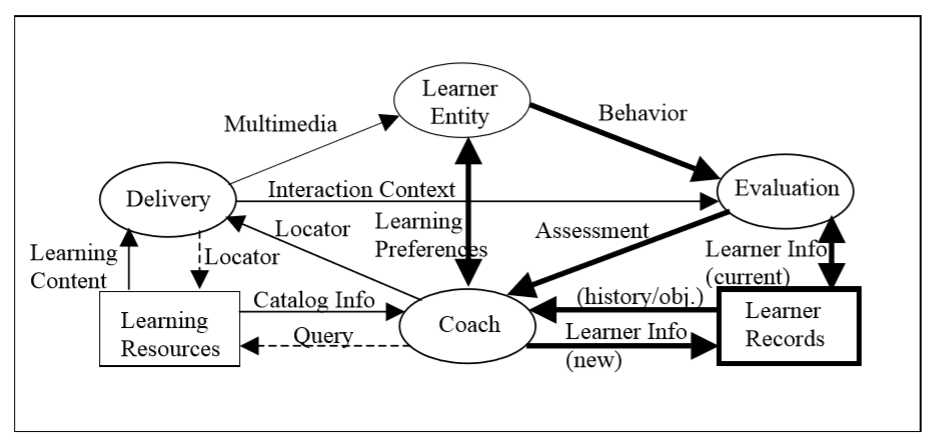
\includegraphics[width=1.0\textwidth]{LTSA}
    \caption[Learning Technology Systems Architecture]
        {Learning Technology Systems Architecture, IEEE P1484.1/D9 \citep{farance1999learning}}
    \label{fig:LTSA}
\end{figure}

E-learning has been growing as an industry and research area, and various standards have been devised. One of the most
useful is IEEE P1484.1/D9: the Learning Technology Systems Architecture (LTSA). It provides a valuable way of organising 
the scope and discussion around proposed e-Learning systems, identifying four main components: learner entity, coach, 
delivery and evaluation; and two main resources: learning resources and learner records (See figure \ref{fig:LTSA}).

Identifying what a future, blockchain based system could improve in these critical areas 
can further enhance this project. \citet{garrison2011learning} identified several areas 
that current e-Learning research and practices focus on:

\begin{itemize}
    \item Enhancing the learning community and social presence
    \item Enhancing the cognitive (practical inquiry and critical thinking) presence, 
    especially with asynchronous (pre-recorded)
    \item Self-regulation and motivation: a self-regulated learner achieves more
    \item 
\end{itemize}

\subsection{Self-Regulation and Motivation}

% There are several dimensions of self-regulation that will help a learner stay on an 
% e-Learning course or curriculum:

% \begin{table}[!ht] 
%     \caption{Self-Regulation and Motivation Strategies, adapted from \citep[p.189]{o2013web}}
%     \centering
%     \label{table:good_table}
%     \begin{tabular}{l c }
%         \toprule
%         Self-regulation dimensions & Examples of Motivation Strategies \\ 
%         \midrule
%         Motives & Setting challenging but achievable goals \\ \hline
%         Methods of Learning & Summarisation, outline-formatted notes, \\
%         & interrogation and rehearsal, etc\\ \hline
%         Time Management & Prioritizing tasks, dealing with procrastination\\ \hline
%         Physical Environment & An environment conducive to learning\\ \hline
%         Social environment & Help seeking: knowing when help is needed,\\
%         & identifying sources of help, framing help request,\\
%         & evaluating help received\\ \hline
%         Performance & Observing and reflecting upon performance\\
%         & with short-term and long-term goals\\
%         \bottomrule
%     \end{tabular}
% \end{table}

An e-learning programme should equip a learner with these self-regulation skills,
and the e-learning system should provide tools that facilitate and enable the 
motivation strategies.

\subsection{Security and Privacy}

The security of e-learning systems have also been a concern. For example, \citet{el2003privacy} noted that “While many 
advances have been made in the mechanics of providing online instruction, the needs for privacy and security have to-date 
been largely ignored. At best they have been accommodated in an ad-hoc, patchwork fashion.” 

\section{Properties of Blockchain Technologies}

Impossible to collude: executed by transparent code, increase trust and enables reputation building for even new entrants to 
the education market
Protects learner: guaranteed records and rewards
% Scam? Reputation building? https://books.google.co.uk/books?id=jEsRVTbukyMC&lpg=PR5&ots=DKQbVRC8Yh&dq=high%20education%20assessment%20reputation&lr&pg=PA233#v=onepage&q=high%20education%20assessment%20reputation&f=false
Administration costs of higher education
Smart Contract: secure and cutting the middleman

Characteristics of a blockchain ledger such as Hyperledger:
1. Shared Ledger: 
shared across education and government authorities
2. Smart Contract: 
Swan (2015, p.62) proposed that “rules embedded in learning smart contracts could automatically confirm the completion of learning modules 
through standardized online tests”.
3. Privacy: 
a. Appropriate Visibility
b. Transactions are secure, authenticated and verifiable
4. Consensus: All shared ledger parties agree to transactions

Openness and transparency of online courses and online assessments is encouraged: using an interpreted language, instead of a compiled 
one, to write the smart contract, so the actual code is visible on the blockchain and can be easily inspected
% Trust in Education Providers can be maintained the identity of any addition or modification to the record can be traced, records cannot 
be removed or altered
% Privacy of course participants is protected: events are publicly-accessible, but not publicly readable without a digital key
Resilient to loss of infrastructure: records are distributed over a network of participating computers

\section{Existing Efforts in Blockchain for Education}

% chapter 1
% The potential of blockchain enabled systems in education has been noted by the community, with \citet[p.62]{swan2015blockchain} 
% proposing that “learning smart contracts could automatically confirm the completion of learning modules through standardized 
% online tests”. Appropriate configurations in permissions and visibility can also provide improved security and privacy to e-Learning.

\subsection{Blockcerts}

A current blockchain in education use case: Blockcerts
Blockcerts is an MIT backed open standard for blockchain certificates. Education providers can use it to store the records of 
certifications they have awarded, in a way where they are immutable and decentralised. 

\subsection{OpenLearn}


% Uncomment this line, when you have siunitx package loaded.
%The SI Units for dynamic viscosity is \si{\newton\second\per\metre\squared}.
% I'm going to randomly include a picture Figure~\ref{fig:minion}.


% If you have trouble viewing this document contact Krishna at: \href{mailto:kks32@cam.ac.uk}{kks32@cam.ac.uk} or raise an issue at \url{https://github.com/kks32/phd-thesis-template/}


% \begin{figure}[htbp!] 
% \centering    
% 
\includegraphics[width=1.0\textwidth]{minion}
% \caption[Minion]{This is just a long figure caption for the minion in Despicable Me from Pixar}
% \label{fig:minion}
% \end{figure}


% \section*{Enumeration}
% Lorem ipsum dolor sit amet, consectetur adipiscing elit. Sed vitae laoreet lectus. Donec lacus quam, malesuada ut erat vel, consectetur eleifend tellus. Aliquam non feugiat lacus. Interdum et malesuada fames ac ante ipsum primis in faucibus. Quisque a dolor sit amet dui malesuada malesuada id ac metus. Phasellus posuere egestas mauris, sed porta arcu vulputate ut. Donec arcu erat, ultrices et nisl ut, ultricies facilisis urna. Quisque iaculis, lorem non maximus pretium, dui eros auctor quam, sed sodales libero felis vel orci. Aliquam neque nunc, elementum id accumsan eu, varius eu enim. Aliquam blandit ante et ligula tempor pharetra. Donec molestie porttitor commodo. Integer rutrum turpis ac erat tristique cursus. Sed venenatis urna vel tempus venenatis. Nam eu rhoncus eros, et condimentum elit. Quisque risus turpis, aliquam eget euismod id, gravida in odio. Nunc elementum nibh risus, ut faucibus mauris molestie eu.
%  Vivamus quis nunc nec nisl vulputate fringilla. Duis tempus libero ac justo laoreet tincidunt. Fusce sagittis gravida magna, pharetra venenatis mauris semper at. Nullam eleifend felis a elementum sagittis. In vel turpis eu metus euismod tempus eget sit amet tortor. Donec eu rhoncus libero, quis iaculis lectus. Aliquam erat volutpat. Proin id ullamcorper tortor. Fusce vestibulum a enim non volutpat. Nam ut interdum nulla. Proin lacinia felis malesuada arcu aliquet fringilla. Aliquam condimentum, tellus eget maximus porttitor, quam sem luctus massa, eu fermentum arcu diam ac massa. Praesent ut quam id leo molestie rhoncus. Praesent nec odio eget turpis bibendum eleifend non sit amet mi. Curabitur placerat finibus velit, eu ultricies risus imperdiet ut. Suspendisse lorem orci, luctus porta eros a, commodo maximus nisi.

% Nunc et dolor diam. Phasellus eu justo vitae diam vehicula tristique. Vestibulum vulputate cursus turpis nec commodo. Etiam elementum sit amet erat et pellentesque. In eu augue sed tortor mollis tincidunt. Mauris eros dui, sagittis vestibulum vestibulum vitae, molestie a velit. Donec non felis ut velit aliquam convallis sit amet sit amet velit. Aliquam vulputate, elit in lacinia lacinia, odio lacus consectetur quam, sit amet facilisis mi justo id magna. Curabitur aliquet pulvinar eros. Cras metus enim, tristique ut magna a, interdum egestas nibh. Aenean lorem odio, varius a sollicitudin non, cursus a odio. Vestibulum ante ipsum primis in faucibus orci luctus et ultrices posuere cubilia Curae; 
% \begin{enumerate}
% \item The first topic is dull
% \item The second topic is duller
% \begin{enumerate}
% \item The first subtopic is silly
% \item The second subtopic is stupid
% \end{enumerate}
% \item The third topic is the dullest
% \end{enumerate}
% Morbi bibendum est aliquam, hendrerit dolor ac, pretium sem. Nunc molestie, dui in euismod finibus, nunc enim viverra enim, eu mattis mi metus id libero. Cras sed accumsan justo, ut volutpat ipsum. Nam faucibus auctor molestie. Morbi sit amet eros a justo pretium aliquet. Maecenas tempor risus sit amet tincidunt tincidunt. Curabitur dapibus gravida gravida. Vivamus porta ullamcorper nisi eu molestie. Ut pretium nisl eu facilisis tempor. Nulla rutrum tincidunt justo, id placerat lacus laoreet et. Sed cursus lobortis vehicula. Donec sed tortor et est cursus pellentesque sit amet sed velit. Proin efficitur posuere felis, porta auctor nunc. Etiam non porta risus. Pellentesque lacinia eros at ante iaculis, sed aliquet ipsum volutpat. Suspendisse potenti.

% Ut ultrices lectus sed sagittis varius. Nulla facilisi. Nullam tortor sem, placerat nec condimentum eu, tristique eget ex. Nullam pretium tellus ut nibh accumsan elementum. Aliquam posuere gravida tellus, id imperdiet nulla rutrum imperdiet. Nulla pretium ullamcorper quam, non iaculis orci consectetur eget. Curabitur non laoreet nisl. Maecenas lacinia, lorem vel tincidunt cursus, odio lorem aliquet est, gravida auctor arcu urna id enim. Morbi accumsan bibendum ipsum, ut maximus dui placerat vitae. Nullam pretium ac tortor nec venenatis. Nunc non aliquet neque. 

% \section*{Itemize}
% \begin{itemize}
% \item The first topic is dull
% \item The second topic is duller
% \begin{itemize}
% \item The first subtopic is silly
% \item The second subtopic is stupid
% \end{itemize}
% \item The third topic is the dullest
% \end{itemize}

% \section*{Description}
% \begin{description}
% \item[The first topic] is dull
% \item[The second topic] is duller
% \begin{description}
% \item[The first subtopic] is silly
% \item[The second subtopic] is stupid
% \end{description}
% \item[The third topic] is the dullest
% \end{description}


% \clearpage

% \tochide\section{Hidden section}
% \textbf{Lorem ipsum dolor sit amet}, \textit{consectetur adipiscing elit}. In magna nisi, aliquam id blandit id, congue ac est. Fusce porta consequat leo. Proin feugiat at felis vel consectetur. Ut tempus ipsum sit amet congue posuere. Nulla varius rutrum quam. Donec sed purus luctus, faucibus velit id, ultrices sapien. Cras diam purus, tincidunt eget tristique ut, egestas quis nulla. Curabitur vel iaculis lectus. Nunc nulla urna, ultrices et eleifend in, accumsan ut erat. In ut ante leo. Aenean a lacinia nisl, sit amet ullamcorper dolor. Maecenas blandit, tortor ut scelerisque congue, velit diam volutpat metus, sed vestibulum eros justo ut nulla. Etiam nec ipsum non enim luctus porta in in massa. Cras arcu urna, malesuada ut tellus ut, pellentesque mollis risus.Morbi vel tortor imperdiet arcu auctor mattis sit amet eu nisi. Nulla gravida urna vel nisl egestas varius. Aliquam posuere ante quis malesuada dignissim. Mauris ultrices tristique eros, a dignissim nisl iaculis nec. Praesent dapibus tincidunt mauris nec tempor. Curabitur et consequat nisi. Quisque viverra egestas risus, ut sodales enim blandit at. Mauris quis odio nulla. Cras euismod turpis magna, in facilisis diam congue non. Mauris faucibus nisl a orci dictum, et tempus mi cursus.

% Etiam elementum tristique lacus, sit amet eleifend nibh eleifend sed \footnote{My footnote goes blah blah blah! \dots}. Maecenas dapibu augue ut urna malesuada, non tempor nibh mollis. Donec sed sem sollicitudin, convallis velit aliquam, tincidunt diam. In eu venenatis lorem. Aliquam non augue porttitor tellus faucibus porta et nec ante. Proin sodales, libero vitae commodo sodales, dolor nisi cursus magna, non tincidunt ipsum nibh eget purus. Nam rutrum tincidunt arcu, tincidunt vulputate mi sagittis id. Proin et nisi nec orci tincidunt auctor et porta elit. Praesent eu dolor ac magna cursus euismod. Integer non dictum nunc.


% \begin{landscape}

% \section*{Subplots}
% I can cite Wall-E (see Fig.~\ref{fig:WallE}) and Minions in despicable me (Fig.~\ref{fig:Minnion}) or I can cite the whole figure as Fig.~\ref{fig:animations}


% \begin{figure}
%   \centering
%   \begin{subfigure}[b]{0.3\textwidth}
%     
\includegraphics[width=\textwidth]{TomandJerry}
%     \caption{Tom and Jerry}
%     \label{fig:TomJerry}   
%   \end{subfigure}             
%   \begin{subfigure}[b]{0.3\textwidth}
%     
\includegraphics[width=\textwidth]{WallE}
%     \caption{Wall-E}
%     \label{fig:WallE}
%   \end{subfigure}             
%   \begin{subfigure}[b]{0.3\textwidth}
%     
\includegraphics[width=\textwidth]{minion}
%     \caption{Minions}
%     \label{fig:Minnion}
%   \end{subfigure}
%   \caption{Best Animations}
%   \label{fig:animations}
% \end{figure}


% \end{landscape}
